\documentclass[11pt]{article}
\usepackage[paperwidth=13.333in,paperheight=7.5in,margin=0.25in]{geometry}
\pagestyle{empty}
\usepackage{tikz}
\usetikzlibrary{arrows.meta,positioning,fit,calc,shapes.geometric,backgrounds}
\usepackage{xcolor}
% The default palette is the white-background evidence-report style. The
% figure builder defines \DARKTHEME for slide-ready variants.
\ifdefined\DARKTHEME
\definecolor{ink}{HTML}{F3F7FA}
\definecolor{muted}{HTML}{B9C7D4}
\definecolor{grid}{HTML}{2B3B4B}
\definecolor{blue}{HTML}{62B8FF}
\definecolor{teal}{HTML}{55D6C2}
\definecolor{orange}{HTML}{FFBD5A}
\definecolor{red}{HTML}{FF7568}
\definecolor{purple}{HTML}{C3A6FF}
\definecolor{paleBlue}{HTML}{14283A}
\definecolor{paleOrange}{HTML}{3A2B14}
\definecolor{dataFill}{HTML}{241C3A}
\definecolor{modelFill}{HTML}{12352F}
\definecolor{specialistFill}{HTML}{3A2B14}
\definecolor{futureFill}{HTML}{1C2630}
\definecolor{pageBg}{HTML}{080D13}
\else
\definecolor{ink}{HTML}{102A43}
\definecolor{muted}{HTML}{52606D}
\definecolor{grid}{HTML}{D9E2EC}
\definecolor{blue}{HTML}{1976A8}
\definecolor{teal}{HTML}{16817A}
\definecolor{orange}{HTML}{D9822B}
\definecolor{red}{HTML}{C05640}
\definecolor{purple}{HTML}{6B5B95}
\definecolor{paleBlue}{HTML}{E8F1F5}
\definecolor{paleOrange}{HTML}{FFF1DF}
\definecolor{dataFill}{HTML}{F5F0FA}
\definecolor{modelFill}{HTML}{EAF6F4}
\definecolor{specialistFill}{HTML}{FFF1DF}
\definecolor{futureFill}{HTML}{F2F4F5}
\definecolor{pageBg}{HTML}{FFFFFF}
\fi
\pagecolor{pageBg}
\tikzset{
  base/.style={font=\sffamily, text=ink},
  title/.style={base, font=\sffamily\bfseries\fontsize{23}{27}\selectfont},
  subtitle/.style={base, font=\sffamily\fontsize{12}{15}\selectfont, text=muted},
  box/.style={base, rounded corners=3pt, draw=blue!65!black, fill=paleBlue, minimum height=0.78cm, minimum width=2.65cm, align=center, inner sep=7pt},
  data/.style={box, draw=purple!75!black, fill=dataFill},
  model/.style={box, draw=teal!75!black, fill=modelFill},
  specialist/.style={box, draw=orange!85!black, fill=specialistFill},
  future/.style={box, draw=muted, fill=futureFill, dashed},
  arrow/.style={-{Latex[length=3mm]}, line width=0.9pt, draw=muted},
  dashedarrow/.style={-{Latex[length=3mm]}, line width=0.8pt, draw=muted, dashed},
  note/.style={base, font=\sffamily\fontsize{18}{22}\selectfont, text=muted, align=left},
}

\begin{document}
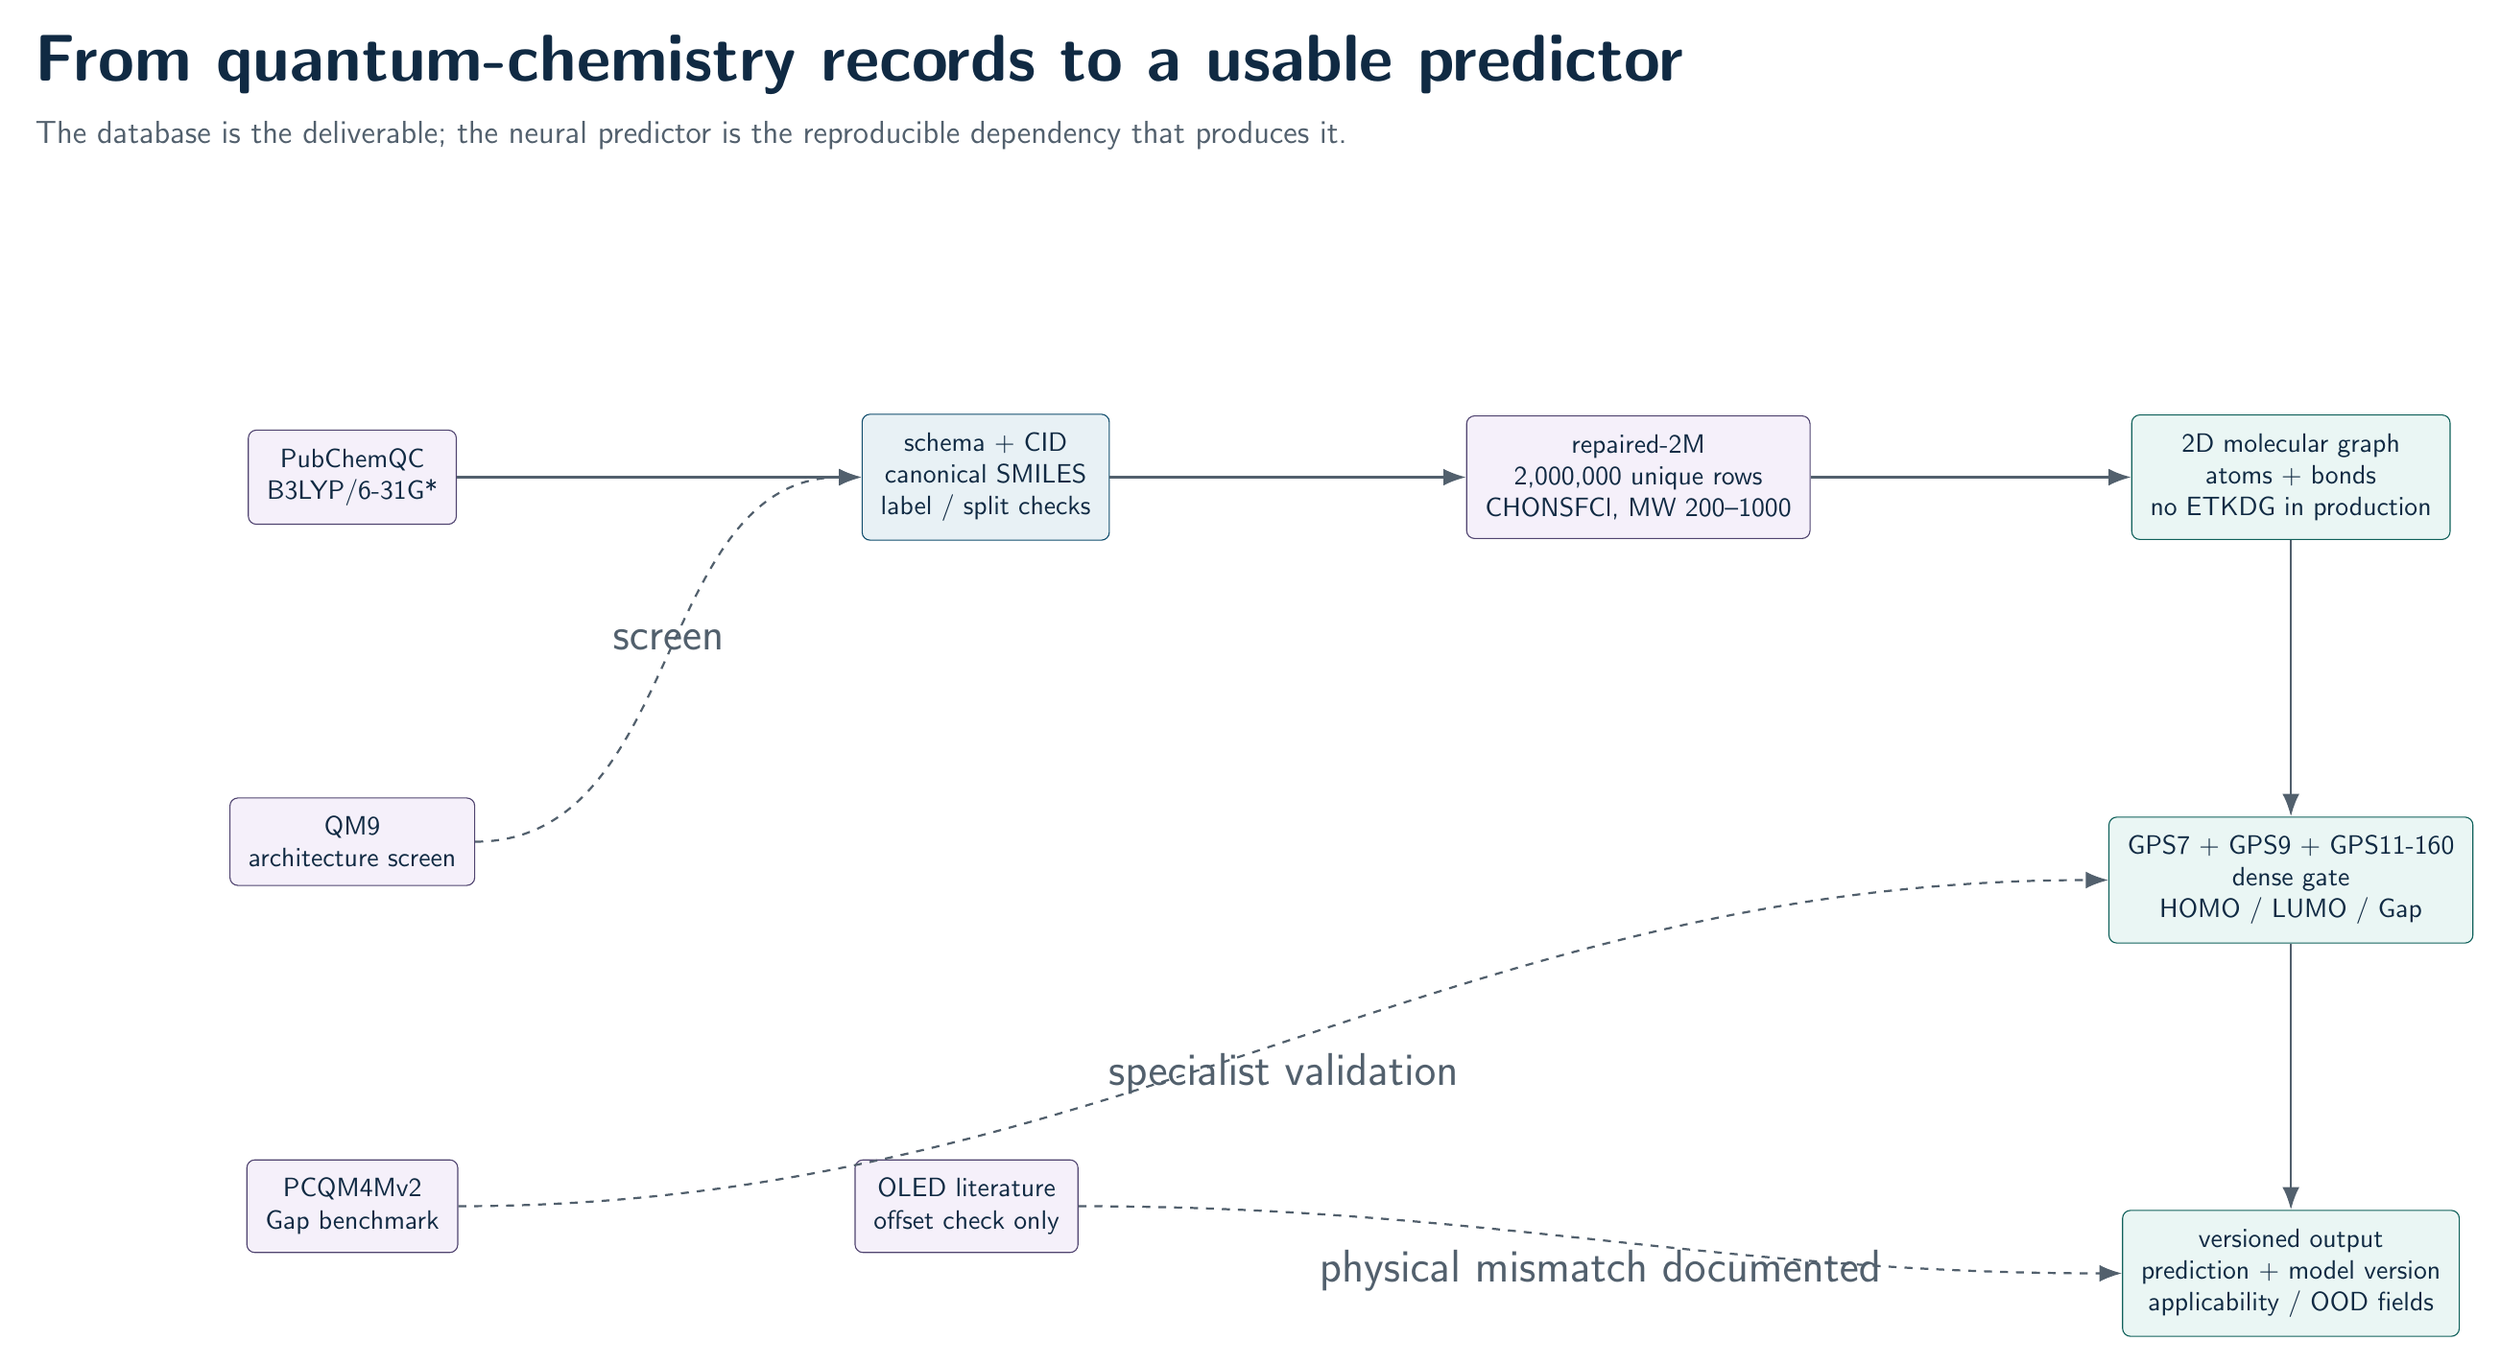
\begin{tikzpicture}[x=1in,y=1in]
  \node[title,anchor=west] at (0,6.85) {From quantum-chemistry records to a usable predictor};
  \node[subtitle,anchor=west] at (0,6.48) {The database is the deliverable; the neural predictor is the reproducible dependency that produces it.};

  \node[data,minimum width=2.55cm,minimum height=1.0cm] (pc) at (1.7,4.7) {PubChemQC\\B3LYP/6-31G*};
  \node[data,minimum width=2.55cm,minimum height=1.0cm] (qm) at (1.7,2.8) {QM9\\architecture screen};
  \node[data,minimum width=2.55cm,minimum height=1.0cm] (pcqm) at (1.7,0.9) {PCQM4Mv2\\Gap benchmark};
  \node[data,minimum width=2.55cm,minimum height=1.0cm] (oled) at (4.9,0.9) {OLED literature\\offset check only};

  \node[box,minimum width=2.9cm,minimum height=1.15cm] (gate) at (5.0,4.7) {schema + CID\\canonical SMILES\\label / split checks};
  \node[data,minimum width=3.0cm,minimum height=1.15cm] (repair) at (8.4,4.7) {repaired-2M\\2,000,000 unique rows\\CHONSFCl, MW 200--1000};
  \node[model,minimum width=3.0cm,minimum height=1.15cm] (graph) at (11.8,4.7) {2D molecular graph\\atoms + bonds\\no ETKDG in production};
  \node[model,minimum width=3.0cm,minimum height=1.15cm] (pred) at (11.8,2.6) {GPS7 + GPS9 + GPS11-160\\dense gate\\HOMO / LUMO / Gap};
  \node[model,minimum width=3.0cm,minimum height=1.15cm] (db) at (11.8,0.55) {versioned output\\prediction + model version\\applicability / OOD fields};

  \draw[arrow] (pc.east) -- (gate.west);
  \draw[arrow] (gate.east) -- (repair.west);
  \draw[arrow] (repair.east) -- (graph.west);
  \draw[arrow] (graph.south) -- (pred.north);
  \draw[arrow] (pred.south) -- (db.north);
  \draw[dashedarrow] (qm.east) to[out=0,in=180] node[above,note] {screen} (gate.west);
  \draw[dashedarrow] (pcqm.east) to[out=0,in=180] node[below,note] {specialist validation} (pred.west);
  \draw[dashedarrow] (oled.east) to[out=0,in=180] node[below,note] {physical mismatch documented} (db.west);
\end{tikzpicture}
\end{document}
